\documentclass[11pt,a4paper]{report}
\usepackage[english]{babel}
\usepackage[utf8]{inputenc}
\usepackage[T1]{fontenc}
\usepackage{glossaries}
\usepackage{graphicx}
\usepackage{hyperref}
\usepackage{wrapfig}
\usepackage{float}
\usepackage{natbib}
\usepackage{listings}
\usepackage{caption}
\usepackage{subcaption}
\newcommand{\HRule}{\rule{\linewidth}{0.5mm}}
\setlength\parindent{0pt} % Removes all indentation from paragraphs	 
%% Acronimos
%\newglossaryentry{sqlite}
%{
%  name=SQLite,
%  description={é um sistema de gestão de base de dados}
%}
%\newacronym{aes}{AES}{Advanced Encryption Standard}
%\newacronym{sha}{SHA}{Secure Hash Algorithm}
%\makeglossaries
%% Fim da introdução do Acronimos

\let\olditemize\itemize
\renewcommand{\itemize}{
  \olditemize
  \setlength{\itemsep}{1pt}
  \setlength{\parskip}{0pt}
  \setlength{\parsep}{0pt}
}

\title{\textbf{Identity Enabled Distribution Control System} \\1st Project\\ Segurança\\Universidade de Aveiro}
\author{Diogo Silva 60337 \and Tânia Alves 60340 }

\begin{document}
\begin{titlepage}
\begin{center}
\HRule \\[0.4cm]
{ \huge \bfseries Identity Enabled Distribution Control System \\[0.4cm] }
\HRule \\[1.5cm]
\textsc{\LARGE Universidade de Aveiro}\\[1.5cm]
\textsc{}\\[1.5cm]
\textsc{Diogo Silva 60337 \\Tânia Alves 60340 }
\end{center}
\end{titlepage}
\maketitle
\tableofcontents
\nocite{*}
\chapter*{Context}
\addcontentsline{toc}{chapter}{Context}
This project was done for Security, for the 2015/2016 lective year.
It aims to create an end to end secure digital rights management system to handle the distribution of video files, music files or books.

\chapter*{Introduction}
\addcontentsline{toc}{chapter}{Introduction}

Our project is made of two main components: the player and the server.
The server is in charge of controlling the user access to the protected files. 
The player requests and plays the files from the server.
In order for the user to have access to the titles he/she wants, we also have a web application where the user can buy the titles to play later.
To reach the goal of this project, we also needed a database that helped manage the user and file related information.

\begin{figure}[H]
\centerline{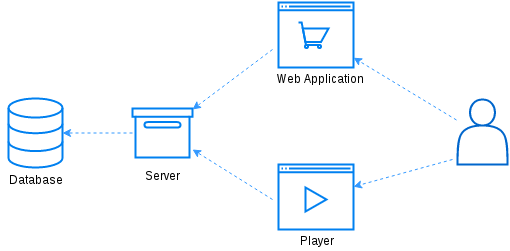
\includegraphics[width=300pt]{images/overview.png}}
\caption{Component overview}
\label{schema}
\end{figure}

%%%% CAPITULO RELATIVO A APLICAÇÃO %%%%
\chapter{System components}
This chapter includes information about the database we used to support the server.
We stored information about the users, files, players and devices that were later used.

\section{Database}
For the database we thought of this layout:

\begin{figure}[H]
\centerline{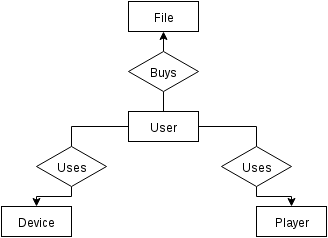
\includegraphics[width=200pt]{images/dbSchema.png}}
\caption{DB Schema}
\label{schema}
\end{figure}

We need to save information about the users that belong to the system and buy the files. 
The files that are stored in the server and are then sent to the players. The players that will interact with the server and play the files. And the devices where the users play the files.

\subsection{Database tables}
Using the information presented, we derived the tables for the database, with all the attributes necessary for our implementation of the system.

\begin{figure}[H]
\centerline{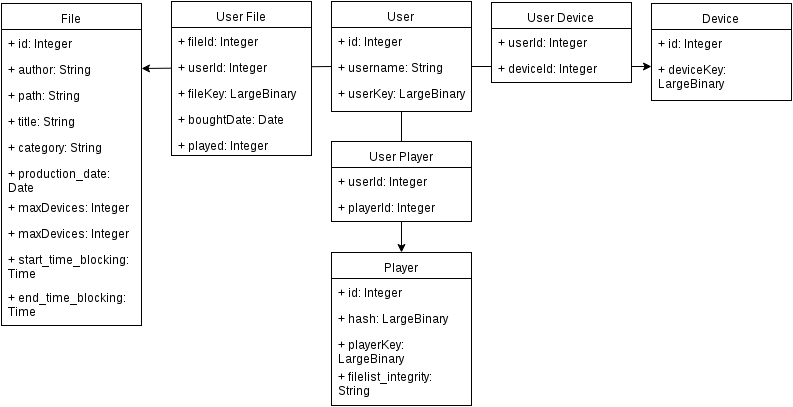
\includegraphics[width=500pt]{images/dbTables.png}}
\caption{DB Tables}
\label{tables}
\end{figure}

Each "main" entities (User, Device, File and Player) will have an id that identifies the entity in the database.
We then have the required key for each one of them as well.
\newline In the User table we have added the username field that identifies the each user.
\newline The File table also has some extra fields that provide information to the user about the file he is playing or buying, such as, the title of the file, the author, the category and the date of the title's production.
\newline The actions presented in Figure 1.1 had to be converted to extra tables since, in each case we had a many-to-many relationship. So, we have here the extra tables that store some information of the interactions, like specific keys and adittional information like the date that when the user bought the file. 
\newline Besides the tables presented before, we needed a few more tables to help implement the authorization policies:

\begin{figure}[H]
\centerline{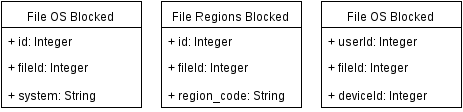
\includegraphics[width=300pt]{images/auxTables.png}}
\caption{DB Auxiliary Tables}
\label{tables}
\end{figure}


\subsection{Technologies used}
For the database we used:
\begin{description}
  \item[PostgreSQL] Open source, object relational database management system. We chose this over SQLite for example because it has a better support for storing secure data.
  \item[SQLAlchemy] Open source SQL toolkit. Works as an object-relation mapper for Python. This allowed us to create database scripts that created the tables and populated the database.
\end{description}

\section{Server}
The server is meant to interact with the database and control the access of the users and players to the files.
This interaction is done over a \emph{HTTP Rest} interface.
 
\subsection{Structure}
The server is composed of several files:

\begin{description}
  \item[Server file] This is the main file that holds the code to execute the server. When we want to start the server, it must be with \emph{sudo} because server is using port 443 to host (which requires previligies).
  \item[Custom adapter file] This is the file that overrides the BuiltinSSL class developed by CherryPy, default adapter doesn't support certificate peer verification and it is useful to check if player is valid and associate it with a determined key.
  \item[Cipher file] This file holds auxiliary cryptographic functions that are used by the server.
  \item[Checker file] Holds auxiliary functions that make certain verifications before each request to the \emph{HTTP Rest API}, such as making sure the user is logged in before the player tries to download a file, or check if there's a device key reported when player logged in, etc.
\end{description}

\subsection{Implementation}
The server communicates with the player through \emph{SSL}. We did it like this so that we could focus on other parts of the system instead of implementing it from scratch.
For this, we needed to create certificates for both server and players.

\subsection{Technologies used}
\begin{description}
  \item[CherryPy] Object oriented web application framework for Python. We chose this because it is built for rapid development of web applications and offers the basic configurations, that is what were looking for.
  \item[psycopg2 package] This is a Python-PostgreSQL database adapter that manages context, diagnosis erros and more.
  \item[OpenSSL] Toolkit that implements SSL and TLS protocols with cryptographic support. We used this so that we could create a certain level of abstraction on how the communications were made, and like that, we could focus in the rest of the system.
\end{description}

\section{Web page}
The web page is where the user can buy the titles.
It requires the user to log in before proceeding with the titles purchase.
The same API that the player uses is used here.

\begin{figure}[H]
\centerline{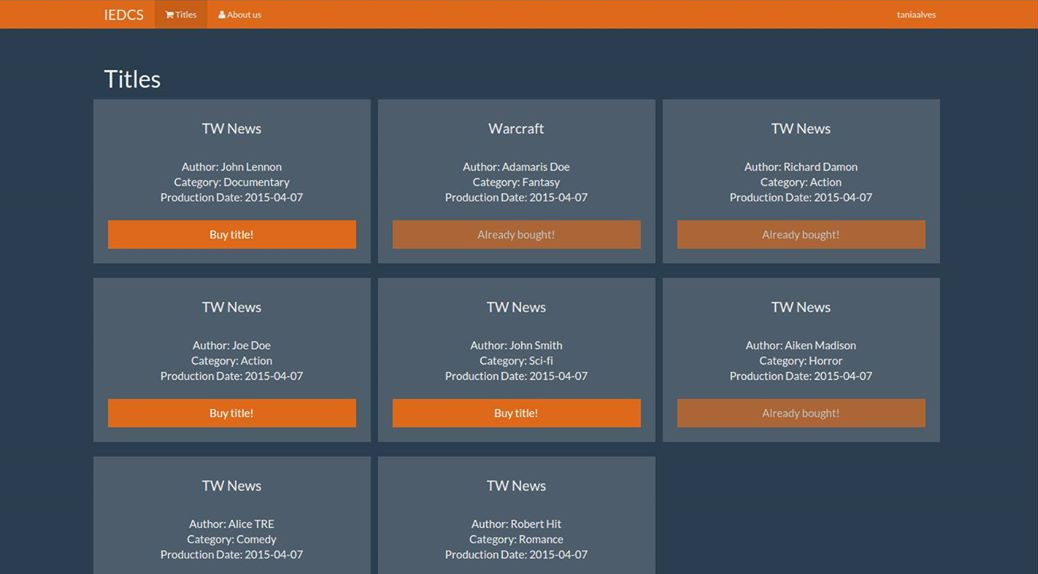
\includegraphics[width=500pt]{images/webpage.jpg}}
\caption{Web page interface}
\label{webpage}
\end{figure}

It is a simple interface that has a button to buy a specific title.

\section{Player}
The player allows the user to play the files he/she has bought previously. 
\newline  In this implementation we used video files in order to prove that our implementation can handle big files.

\subsection{Structure}
The player implementation we have is made of 3 main files. 

\begin{description}
  \item[Player file] This file contains the mainloop for the player's graphical interface. It is here where most of the requests to the server and main operations are made.
  \item[Playback file] The playback file contains the code that actually plays the file. The decryption is done here, block by block and fed to the thread that runs a VLC player instance..
  \item[My List file] This file is an auxiliary file that defines the structure of the list that the player displays to the user containing the titles the users owns. This is only to improve the appeareance of the list.
  \item[videos folder] This folder is where the player stores the encrypted videos. Inside, there is another folder for each user that uses the player named after his/her username. This method was chosen so that it is easy for each player to go and grab the files that belong to him/her if he/she chooses to move the files and use another player or device.
  \item[Python requests package] This package enabled us to build the requests and responses to perform the communication.
  \item[PyCrypto package] This is the package that helps handle encryptions and decryptions.
\end{description}

\subsection{Implementation}
After the user starts the player application, he/she must log in. 

\begin{figure}[H]
\centerline{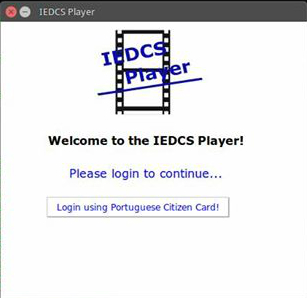
\includegraphics[width=200pt]{images/playerLogin.jpg}}
\caption{Login page for the player}
\label{player}
\end{figure}

At this stage, the only information required to perform the login is the username. Further along the road, the login will also be possible using the Portuguese Citizen Card.
\newline After the user logs in and it is confirmed by the server, a list of titles is displayed so that the user can choose which one he/she wants to reproduce.

\begin{figure}[H]
\centerline{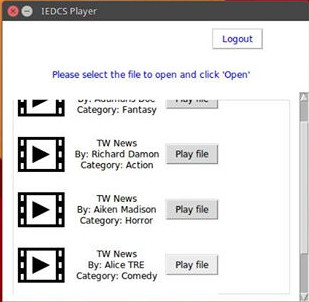
\includegraphics[width=200pt]{images/playerList.jpg}}
\caption{Page that lists the files for the user}
\label{player}
\end{figure}

When the user selects the file that he/she wants to play, a thread running the VLC player is started. The thread reads blocks of the encrypted file, decrypts it and sends it to the VLC buffer.
\newline
The buffer is managed by the VLC player and is customizable (the user can give the buffer the size it wants by changing the value on the VLC settings).

\begin{figure}[H]
\centerline{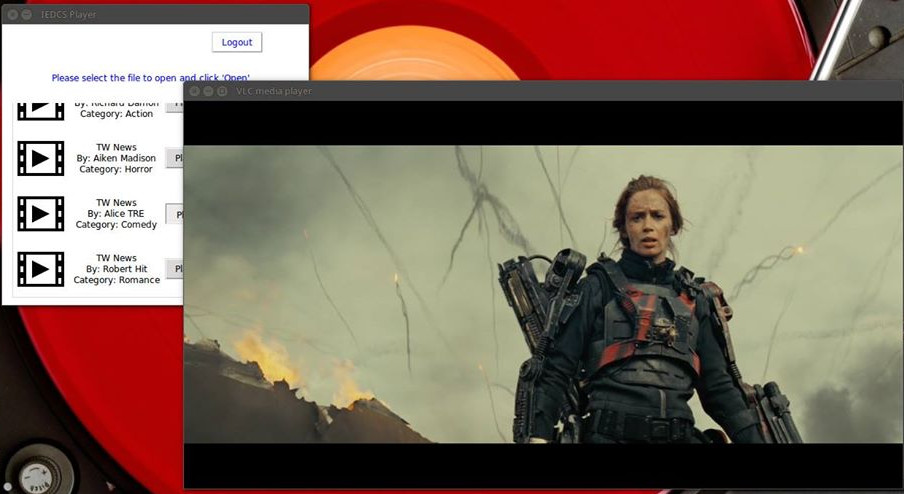
\includegraphics[width=300pt]{images/playerPlay.jpg}}
\caption{Video playing in the VLC thread}
\label{player}
\end{figure}


All the requests done to the server are performed over the server's \emph{HTTP Rest} API that was presented earlier.

\subsection{Technologies used}
\begin{description}
  \item[Tkinter] We built the graphical interface with Tkinter that is the Python graphic user interface framework.
  \item[VLC Player] To make things a bit easier when handling video files, we used the VLC player that takes care of the video format encoding.
  \item[Python requests package] This package enabled us to communicate with the server producing requests and receiving responses.
  \item[PyCrypto package] This is the package that helps handle encryptions and decryptions.
\end{description}

\chapter{System keys}
\section{Player Key}
This is a key that must be generated after each code is evaluated by the company that wants to implement the system. 
This evaluation checks if the player, and the respective code, meet the security requirements. 
Taking into consideration when it is generated and the process behind it, this key ensures that the player works accordingly to the security policies.
\newline At this stage, the player was generated from a random array of bytes and stored in the database, on the server side, since we are the ones that are devoloping the player.
In the player, the Player Key is hardcoded.
\newline This key is present in the server and in the player.

\section{Device Key}
The Device Key is a key that identifies the device where the player is being executed. This key should be the same even if the we have more than one player running in a device.
In the Device Key generation, there were some dificulties in finding the best solution.
\newline We wanted to use the processor serial number because we know that the number we get is already unique.
However, this is an information that is hard to get. We came across the command \emph{cpuid} that is used in linux systems, but the Python wrapper available, \emph{Pycpuid}, lacks documentation and has incomplete features, making the task of getting the UUID hard. 
\newline We then turned to the command \emph{dmidecode} that gives us a list of device informations that could be used. 
Yet again, we found an obstacle. To access the processor serial number, we needed to run the player with \emph{sudo} which goes against one of the principles of security ("No entity should have greater permissions in the system other than basic permissions it needs to perform its tasks").
So, with some research we found that the information the \emph{dmidecode} command provides is stored in some system files, specifically, in the \emph{/sys/devices/virtual/dmi/id/} directory.
We then browsed all the files present in the directory and came across the one file that didn't require \emph{sudo} to read. 
This file was the \emph{modalias}, that contained all the information gathered by \emph{dmidecode} that didn't require superuser permissions.
\newline So, for the device key generation, we read the file and hashed the entire content with SHA256, using its digest.
\newline In our solution, this key is generated when the user logs in and is sent to the server at this stage. So, the Device Key is present both in the player and in the server.

\section{User Key}
The User Key is a key that identifies the user in the server. 
In our implementation, this key is generated when the user registers in the web page and is then stored in the database along with the rest of the user information gathered.
This key is only ever present in the server, and, as we will see, this will be part of the step that forces the player to communicate with the server each time a file is played.

\section{File Key}
This key identifies the file that the user bought and is independent of the device and player. When compared to the rest of the keys, this one requires a bit more work to derive.

\begin{figure}[H]
\centerline{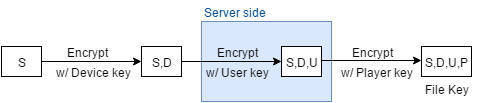
\includegraphics[width=300pt]{images/fileKey.png}}
\caption{Derivation process for the File Key}
\label{fileKey}
\end{figure}

As we can see from the previous diagram, the File Key is derived from the previous keys presented by encrypting them in a chain of operations.
We used the AES algorithm for this.
\newline In the server side, if it is the first file encryption that the server performs for that file and user, we have the following steps:
\begin{enumerate}
  \item The server generates a random start seed.
  \item It then performs the encryption chain presented above to get the resulting File Key.
  \item The server then encrypts the file with the result.
  \item The encrypted file and the start seed are sent to the player so that it can decrypt the file.
  \item The server stores the File Key in the database.
\end{enumerate}

If the file has already been sent at least one time, the steps change a bit:
\begin{enumerate}
  \item The server gets the File Key stored in the database.
  \item It then performs the chain of encryption in reverse, decrypting the File Key with the rest of the keys that it has access at that time.
  \item The result will be the seed that was used to derive that File Key, and so, it is sent to the player.
\end{enumerate}

This chain allows the player to derive the File Key, even if the device changes, because the information that the server sends to the player is the starting seed.
\newline In the player side, whatever the File Key is, the operation's chain is the same. However, the blue square present in the diagram above represents a step in which the player must include the server because it does not have access to the User Key.
\begin{enumerate}
  \item The player gets the seed from the server and encrypts it with the Device Key.
  \item It then sends the result to the server and the server will encrypt it with the User Key, which the player does not have access to.
  \item The server sends the result back and the player will then encrypt it with the Player Key, resulting in the File Key.
\end{enumerate}

\chapter{Server-Client interactions}

\section{Checking player integrity}
Every time a player executes, an operation to check its integrity is performed. This falls into the authorization headers, however, we deal with it right off the start.
We get the files that belong to the player implementation and create a hash of each of the files. We then concatenate the hashes of each file and once more hash the result with a random generated salt and we get the final result.

The server keeps a copy of this result, and, when the player is executed, it will perform the same process. The result will be compared with the information stored in the server, and if they are equal, the player's integrity will be confirmed, otherwise, we assume someone has altered the code and the player is rejected.

\section{Logging in}
To be able to perform any action, the user must first login. This is mandatory in both web page and player.
\newline For this, the server offers a login operation through the \emph{Rest API}

\begin{figure}[H]
\centerline{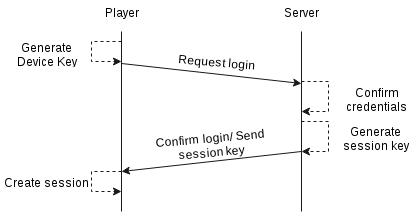
\includegraphics[width=200pt]{images/loginDiagram.png}}
\caption{Login interaction (player - server)}
\label{player}
\end{figure}

As we can see from the diagram above:
\begin{enumerate}
  \item The player starts by generating the Device Key for the device.
  \item The player requests the login from the server, sending it the generated Device Key and the username that the user inserted. 
  \item The server then accesses the database to verify the username it received and associate the Device Key to the user.
  \item The server sends the response that signals the opetaion was completed successfully.
\end{enumerate}

The communication between player and server is done using sessions. Before the player starts communicating with the server, a session is created with the \emph{requests} package for Python.
From now on, all communications will be performed over this session.

\section{Purchasing the file on the web page}
This operation requires the user to be logged in already and is only available in the web page.

\begin{figure}[H]
\centerline{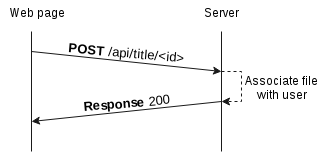
\includegraphics[width=200pt]{images/buyTitle.png}}
\caption{Purchase interaction (player - server)}
\label{player}
\end{figure}

As we can see, the operation isn't complex and the only thing done here is the association of the purchased file with the user.
This association translates in a new entry in the UserFile table in the database.

\section{Downloading the file from the player}
In this interaction, we have two distinct situations:
\begin{enumerate}
  \item Full file download
  \item Cryptographic information download
\end{enumerate}

\subsection{Full file download}
The full file download situation means that this is the first time the player downs the file the user selected.
And so, the server must send back the full encrypted file along with the cryptographic information that will allow the player to decrypt said file.

\begin{figure}[H]
\centerline{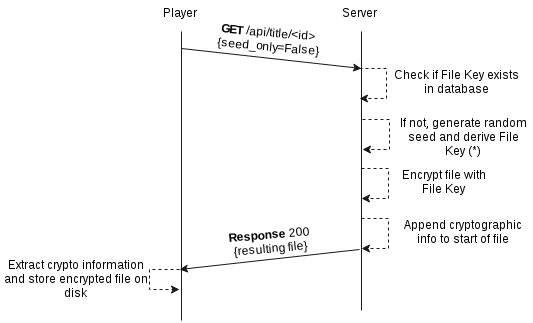
\includegraphics[width=200pt]{images/fullFileDown.png}}
\caption{Full file download (player - server)}
\label{player}
\end{figure}

(*) In this operation, there can be yet another two situations:

\begin{enumerate}
  \item The server has no File Key stored in the database, which forces the server to generate a random start seed to derive the File Key from. It then sends the seed with the encrypted file.
  \item The server already has a File Key stored, and it must derive the starting cryptographic information to send to the player, along with the file.
\end{enumerate}

\subsection{Cryptographic information download}
This situation only occurs if the player has already downloaded the file and has it stored on the disk.

\begin{figure}[H]
\centerline{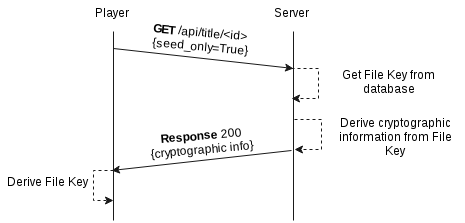
\includegraphics[width=200pt]{images/seedOnlyDown.png}}
\caption{Seed only download (player - server)}
\label{player}
\end{figure}

\section{Logging out from the player}
Logging out is a simple operation that only implies ending the session in the server.

\begin{figure}[H]
\centerline{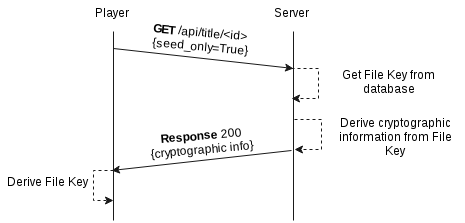
\includegraphics[width=200pt]{images/seedOnlyDown.png}}
\caption{Seed only download (player - server)}
\label{player}
\end{figure}


\chapter{Conclusions}
\section{Encountered problems}
\section{Future work}

%\printglossaries
%\addcontentsline{toc}{chapter}{Glossário}

\bibliographystyle{plain}
\bibliography{proj2}
%\addcontentsline{toc}{chapter}{Bibliografia}

%\listoffigures
%\addcontentsline{toc}{chapter}{Lista de figuras}
%\listoftables
%\addcontentsline{toc}{chapter}{Lista de tabelas}

\end{document}
